\documentclass[runningheads]{llncs}
%
% Compiles with the standard Springer LNCS/CCIS toolchain (llncs.cls +
% splncs04.bst), e.g. via Overleaf's "Springer LNCS" template, or a local
% MiKTeX/TeX Live install. No LaTeX compiler was available in the
% environment this paper was drafted in, so this source has NOT been
% compiled to PDF yet -- compile and proofread page breaks/floats before
% submission.
%
\usepackage{graphicx}
\usepackage{booktabs}
\usepackage{amsmath}
\usepackage{hyperref}

\begin{document}

\title{Burst-Level Data Leakage in Small Hand-Landmark Sign Language
Datasets: A Case Study on a Real-Time Indian Sign Language Recognition System}

% NOTE: placeholder authors/affiliation -- fill in real names before
% submission. Do not invent author identities.
\author{[Author names -- to be completed]}
\institute{[Affiliation -- to be completed]}

\maketitle

\begin{abstract}
We describe a real-time, two-handed Indian Sign Language (ISL) recognition
system built from MediaPipe hand landmarks, a 132-dimensional
scale/position-normalized feature vector, and a Random Forest classifier,
running end-to-end in a browser over a plain webcam. While preparing an
honest evaluation of this system, we found that its data collection
workflow -- a press-and-hold UI that appends dozens of consecutive video
frames to a CSV per recording action, a pattern we believe is common to
small-scale gesture-dataset tools -- produces near-duplicate frames within
each recording action ("burst"). A naive random train/test split, the
default in the system's own original training code, reports $100.00\%$
held-out accuracy; the same model evaluated with a burst-disjoint split
collapses to $0.00\%$, because in our 842-sample, 18-class dataset nearly
every class was recorded in exactly one continuous burst, so holding a
burst out removes that class from training entirely. That subject/signer-level
train-test leakage inflates reported gesture- and sign-recognition
accuracy is already documented in adjacent literature; our contribution is
narrower and case-study-scoped: we show the same failure recurs one level
below signer granularity, \emph{within} a single signer's own recording
session, propose a lightweight \emph{1-NN same-burst collision rate}
diagnostic for catching it, and are transparent that on our specific
dataset -- where class and recording burst are almost perfectly
confounded -- the diagnostic's near-total collision rate is close to
tautological rather than a surprising empirical finding; its value is as
a pre-flight check applicable to datasets where multiple bursts per class
exist. We instrument the system to record signer/session/burst identity
for every future sample, specify a concrete multi-signer data collection
protocol, and report plainly what can and cannot honestly be claimed from
the current data -- in-sample feature-separability and classifier/latency
comparisons, yes, with the caveat that near-perfect in-sample fit is
expected and uninformative on this data; signer- or session-generalization,
not yet. We offer this as a transparent negative-result case study and a
reusable diagnostic/instrumentation pattern, not as a new
state-of-the-art accuracy claim.

\keywords{Indian Sign Language \and data leakage \and evaluation
methodology \and hand landmarks \and gesture recognition \and
reproducibility}
\end{abstract}

\section{Introduction}

Indian Sign Language (ISL) is used by a substantial deaf and
hard-of-hearing population in India; Census of India (2011) recorded
5.07 million persons with hearing impairment nationally \cite{census2011},
and ISL has its own grammar and vocabulary, independent of any spoken
Indian language. Most hearing people cannot understand it, and
professional interpreters are scarce, which motivates real-time,
camera-only translation tools that need no specialized hardware.

We built such a system: a Flask web application that captures webcam
video, runs MediaPipe's Hand Landmarker on both hands, converts the
21-point-per-hand landmarks into a 132-dimensional, scale- and
position-normalized feature vector, and classifies it with a Random
Forest into one of 35 target classes (26 fingerspelling letters plus 9
common-word gestures), assembling recognized letters into words and
sentences with browser-based text-to-speech output. The system includes a
built-in "Trainer" UI: a user holds a sign for 2--3 seconds while the app
appends every captured frame's feature vector to a CSV, so that anyone can
extend the vocabulary without writing code. The 35-class vocabulary and
interface were designed by the development team without input from Deaf
or hard-of-hearing signers or a certified ISL interpreter; we return to
why that matters for an accessibility-motivated system in Section~7.

That data collection design turned out to have a consequence we had not
anticipated. Because each press-and-hold action appends many
near-identical consecutive frames, and because the shipped training code
used a plain random train/test split, the system's own reported accuracy
was an artifact of matching a test frame to its own near-duplicate
neighbor from the same recording action, not of recognizing the sign. This
paper is the result of auditing that problem rather than reporting past it:
we quantify the leakage precisely, show what an honest evaluation on the
current data can and cannot say, instrument the system to prevent a
repeat, and specify exactly what additional data collection would be
needed for a real signer-generalization claim. We view the diagnostic
methodology -- not a new accuracy number -- as this paper's contribution.

\section{Related Work}

\textbf{ISL and landmark-based sign recognition.} Public ISL resources
have grown recently: iSign \cite{isign2024} is a recent benchmark for ISL
processing, and Patra \emph{et al.} \cite{hwgat2024} introduce a
large-scale isolated-ISL video dataset (2{,}002 words, 40{,}033 videos, 20
signers) together with a hierarchical windowed graph-attention network
over skeleton landmarks. Classical machine learning on hand landmarks
remains an actively published approach for sign recognition generally, not
only for ISL: Random Forest classifiers over landmark or sensor features
have been used for ISL recognition with instrumented gloves
\cite{potluri2021}, and hybrid CNN--Random Forest pipelines over landmark
angles have been proposed for real-time Arabic sign recognition
\cite{arabicslr2024}. Our classifier choice is therefore consistent with,
not a departure from, current practice for small-sample, low-resource sign
recognition.

\textbf{Data leakage from improper evaluation splits.} The general failure
mode we diagnose -- a naive split that leaks correlated samples across
train/test and inflates reported performance -- is a recurring, if
under-cited, problem across sensing-based recognition. Varga
\cite{varga2024} shows that three published WiFi channel-state-information
human action recognition methods report near-$95\%$+ precision under
record-wise splits that collapses substantially once re-evaluated with
subject-disjoint partitioning. Most directly relevant to us, Artiaga
\emph{et al.} \cite{signerdep2025} show that gloss-free sign language
translation models evaluated on PHOENIX14T and CSL-Daily report
substantially degraded BLEU/ROUGE scores under signer-independent,
signer-fold cross-validation compared to the conventional signer-mixed
splits used in prior work, and argue for signer-disjoint evaluation and
explicit reporting of train/test signer overlap as standard practice.

Our work sits one level below these: rather than auditing
\emph{subject}- or \emph{signer}-level leakage in an existing benchmark,
we audit leakage \emph{within a single signer's own data-collection
session}, at the granularity of one continuous recording action. To our
knowledge, no prior sign- or gesture-recognition work formalizes a
same-burst nearest-neighbor collision statistic for this purpose; we
propose one (Section~4) as a lightweight, reusable pre-flight check
applicable to any hand-landmark or pose-based gesture dataset collected
via a press-and-hold or similarly bursty recording UI, of which ours is
unlikely to be the only example.

\section{System Description}

\textbf{Pipeline.} The system runs four cooperating threads connected by
single-slot, drop-oldest queues so that no stage blocks another: a
\emph{grabber} reads and mirrors webcam frames; a \emph{detector} runs
MediaPipe Hand Landmarker (two hands, landmark and presence confidence
thresholds of 0.7) on a resolution-capped copy of each frame and computes
the classifier's prediction; a \emph{renderer} draws the most recently
available hand-landmark overlay onto every captured frame, independent of
how long detection took, so the displayed video framerate does not
degrade under slow detection; and an \emph{encoder} JPEG-compresses frames
for an MJPEG (\texttt{multipart/x-mixed-replace}) stream to the browser.
Decoupling rendering from detection this way (originally the detector
drew directly onto the frame it processed) removed a coupling between
inference latency and perceived video smoothness that is orthogonal to,
but discovered alongside, the leakage issue reported here.

\textbf{Feature representation.} For each detected hand, 21 landmarks
$(x,y,z)$ are translated so the wrist (landmark 0) is the origin and
scaled by the wrist-to-middle-finger-base distance (landmark 9), making
the representation invariant to hand position and distance from the
camera; a hand absent from the frame contributes a zero vector. This
yields 63 features per hand (126 total), to which 6 relative two-hand
features are appended -- the $(\Delta x,\Delta y,\Delta z)$ between
wrists, wrist-to-wrist distance, index-fingertip gap, and thumb-tip gap --
for a 132-dimensional vector intended to let the classifier distinguish
signs that differ only in how the two hands relate to each other (e.g.\
letters that differ by which fingers of one hand touch the other).

\textbf{Classifier and stabilization.} A Random Forest (100 trees, max
depth 15) is trained on these vectors. Because raw per-frame predictions
are noisy during hand transitions, a letter is only committed once its
prediction is the plurality choice for 8 consecutive frames
($\approx 0.27$s at 30fps); this stability gate is a UI/UX filter and is
unrelated to the leakage issue discussed below, which concerns how
training data reaches the classifier, not how its output is smoothed.

\textbf{Static-frame limitation.} All 35 classes, including the 9
"word gesture" classes (e.g.\ \textsc{Hello}, \textsc{ThankYou}), are
classified from a \emph{single} feature vector -- there is no temporal or
trajectory modeling anywhere in the pipeline. Real ISL word signs are
generally motion-based; the system approximates them with one held
key-pose. We flag this as a representational limitation rather than a bug:
it means claims about "gesture recognition" in this system should be
read as static key-pose recognition, not motion recognition.

\section{Diagnosing Burst-Level Leakage}

\textbf{Data collection produces bursts, not independent samples.} The
Trainer UI's press-and-hold action appends one CSV row per captured frame
for the 2--3 seconds the button is held, at the pipeline's capture rate;
we refer to all rows written during one such action as a \emph{burst}.
Prior to this work, the dataset schema recorded only the 132 features and
a class label -- no signer, session, or burst identity was stored, so
bursts could only be reconstructed after the fact.

\textbf{Reconstructing bursts from an unlabeled legacy file.} For the
existing \texttt{isl\_dataset.csv} (842 rows, 18 classes, collected before
this audit), we recovered burst boundaries as maximal runs of
consecutive rows sharing the same label in file order -- a conservative
proxy, since it can only merge two separate recording actions for the
same class into one inferred burst (never split one action into two), so
it cannot manufacture leakage that was not already present. This
recovered 19 bursts across 18 classes: 17 classes were recorded in
exactly one burst each, and one class (\textsc{E}) in two.

\textbf{Quantifying near-duplication.} Within-burst consecutive-frame L2
distances in feature space averaged $0.354$ (median $0.137$; $n{=}823$
pairs), and $14.2\%$ of consecutive within-burst pairs were exact or
near-exact duplicates ($<10^{-6}$ L2 distance) -- both computed across all
18 classes and robust. Cross-burst same-label distances (sampled pairs
from \emph{different} bursts of the same class) averaged $3.032$ (median
$2.124$; $n{=}165$ pairs) -- an $8.6\times$ ratio over the within-burst
figure -- but because only one class (\textsc{E}) has more than one
burst, every one of these 165 cross-burst pairs comes from that single
class; we report the ratio as directionally indicative, not as a
precise, class-balanced estimate, and would not treat it as robust
evidence on its own.

\textbf{The 1-NN same-burst collision rate.} We propose a simple,
reusable diagnostic: for each held-out sample, find its nearest same-label
neighbor in the training set; report the fraction of held-out samples
whose nearest neighbor comes from the \emph{same burst} as itself. A high
rate means a model can score well by matching near-duplicates rather than
by discriminating the sign. Averaged over 20 random 80/20 splits (seeds
0--19, stratified), this rate was $100.0\% \pm 0.0$ (bootstrap 95\% CI
$[100.0\%, 100.0\%]$, computed by resampling the 20 per-seed values) on
our data. We are explicit that this near-total rate is close to
\emph{tautological} here, not a surprising empirical result: with 17 of 18
classes confined to a single burst, a held-out sample's only same-label
training neighbor \emph{can only} come from that one burst by
construction. The diagnostic's intended use is on datasets where classes
have multiple independent bursts (as our proposed collection protocol,
Section~6, would produce), where a high collision rate would be a
genuine, non-tautological warning sign; here it mainly restates, in a
different form, the descriptive fact already visible in
Fig.~\ref{fig:classcounts}'s underlying burst counts. We also note the 20
splits are overlapping resamples of the same 842 rows rather than 20
independent datasets, so their spread understates true variability and
should be read as sensitivity to split randomness, not a sampling-based
confidence estimate.

\section{Experiments}

All experiments run on \texttt{isl\_dataset.csv} as it exists (842
samples, 18/35 target classes populated; 17 classes have zero samples).
Environment: Python 3.14.0, scikit-learn 1.8.0, NumPy 2.4.2, SciPy
1.17.1, Windows 11, Intel Core Ultra 5 125H (CPU only). All numbers are
reproducible via \texttt{evaluate.py} in the project repository.

\subsection{Leakage demonstration}

Table~\ref{tab:leakage} compares a naive random 80/20 stratified split
(matching the system's original training code) against a burst-disjoint
split (\texttt{GroupShuffleSplit} grouped by recovered burst id), both
using the same Random Forest configuration.

\begin{table}[t]
\centering
\caption{Naive vs.\ burst-disjoint evaluation on the same data and model.}
\label{tab:leakage}
\begin{tabular}{lccc}
\toprule
Split & Accuracy & Macro-F1 & Notes \\
\midrule
Naive random 80/20 (stratified) & $100.00\%$ & $1.000$ & matches original code \\
Burst-disjoint (GroupShuffleSplit) & $0.00\%$ & $0.000$ &
4 classes absent from train \\
\bottomrule
\end{tabular}
\end{table}

The naive number is not a measure of sign recognition quality; the
burst-disjoint number is not a measure of poor model quality either --
both are artifacts of a dataset in which (with one exception) every class
has exactly one independent recording session. Repeated over 20 seeds,
the naive split's accuracy was stable at $99.94\% \pm 0.26$ percentage
points (bootstrap 95\% CI $[99.82\%, 100.00\%]$; macro-F1 $1.000 \pm
0.002$), confirming the inflation is systematic, not a lucky split --
though, as noted in Section~4, these 20 splits resample the same 842
rows rather than drawing 20 independent datasets, so this quantifies
sensitivity to split randomness rather than true sampling variance.

\subsection{In-sample classifier and feature comparisons}

Because a valid held-out estimate is not currently obtainable (Section~5.1),
we report in-sample (train-equals-test) comparisons strictly as
capacity/separability diagnostics, \emph{not} generalization estimates.
Table~\ref{tab:classifiers} compares three classifiers trained and
evaluated on the full dataset, including single-sample CPU inference
latency (MediaPipe detection time excluded).

\begin{table}[t]
\centering
\caption{In-sample fit and single-sample inference latency (not a
generalization estimate).}
\label{tab:classifiers}
\begin{tabular}{lcccc}
\toprule
Classifier & In-sample acc. & Macro-F1 & Train (s) & Predict (ms/sample) \\
\midrule
Random Forest (100, depth 15) & $100.0\%$ & $1.000$ & $0.23$ & $37.0$ \\
SVM (RBF, $C{=}10$) & $100.0\%$ & $1.000$ & $0.06$ & $0.13$ \\
$k$-NN ($k{=}5$) & $99.8\%$ & $0.998$ & $0.002$ & $12.5$ \\
\bottomrule
\end{tabular}
\end{table}

We include this table for transparency and reproducibility, not because
it is informative: all three classifiers separate the 18 present classes
almost perfectly in-sample, which is the expected, unremarkable result of
fitting near-duplicate-frame data, and no hyperparameter search was run
for any of the three (depth/$C$/$k$ were fixed, not tuned), so this is
not a tuned comparison either. It should be read only as "the feature
representation is separable enough for simple classifiers to fit
degenerate data," not as evidence favoring any classifier for deployment.
Latency figures are single-machine wall-clock measurements with normal
run-to-run variance of a few milliseconds between repeated runs of this
script; all three remain well under a video frame interval regardless.

\begin{table}[t]
\centering
\caption{In-sample feature ablation.}
\label{tab:ablation}
\begin{tabular}{lccc}
\toprule
Feature set & \# features & In-sample acc. & Macro-F1 \\
\midrule
Full (both hands + 6 relative) & 132 & $100.0\%$ & $1.000$ \\
No relative features & 126 & $100.0\%$ & $1.000$ \\
Right hand only & 63 & $95.4\%$ & $0.936$ \\
\bottomrule
\end{tabular}
\end{table}

Table~\ref{tab:ablation} drops to 63 right-hand-only features and sees a
visible in-sample accuracy drop ($100.0\%\to95.4\%$), indicating some
classes in the current label set are not separable from right-hand
landmarks alone even when memorization is trivially available -- weak
supporting evidence for two-hand tracking mattering, though this too is
an in-sample, not generalization, result, and the 126-feature (no
relative-feature) ablation shows no in-sample separability loss, so we
cannot yet claim the 6 relative features specifically are necessary
rather than merely harmless.

Figure~\ref{fig:confmat} shows the in-sample confusion matrix; it had no
off-diagonal errors for the Random Forest at this operating point, i.e.\
it is a separability check that passed, not a source of qualitative
error analysis in the current dataset.

\begin{figure}[t]
\centering
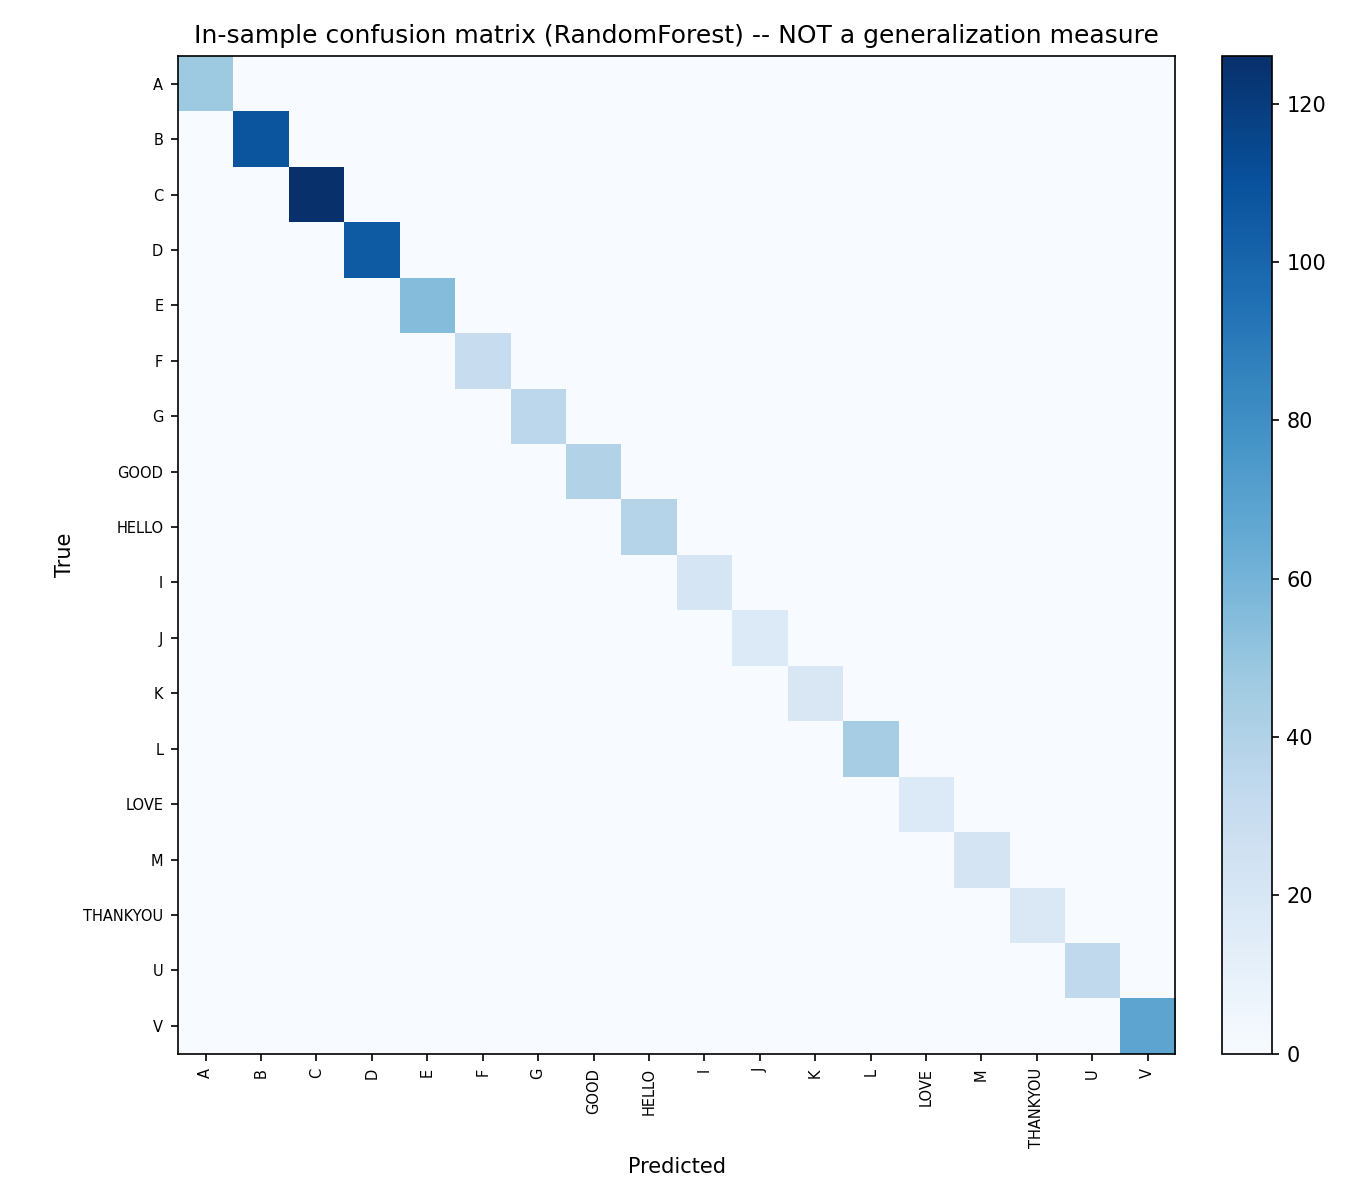
\includegraphics[width=0.75\linewidth]{figs/confusion_matrix.png}
\caption{In-sample confusion matrix (Random Forest). A feature-separability
diagnostic, not a generalization measure.}
\label{fig:confmat}
\end{figure}

\begin{figure}[t]
\centering
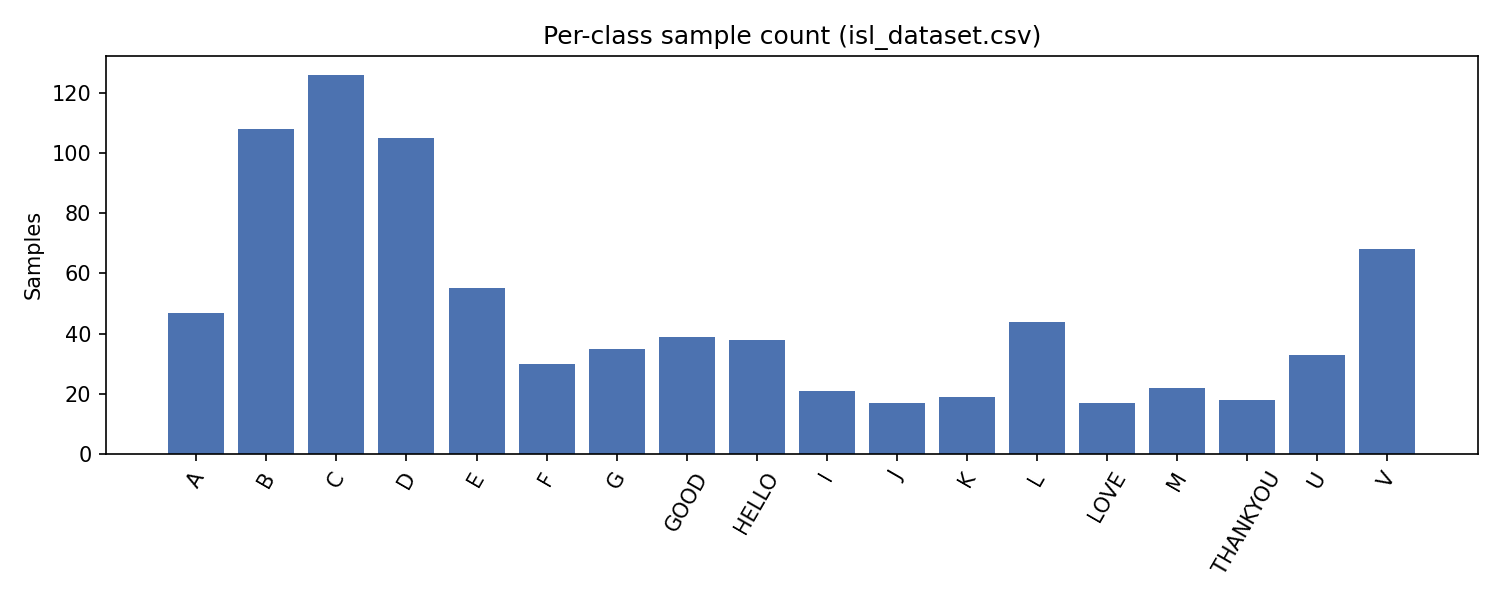
\includegraphics[width=0.9\linewidth]{figs/descriptive_stats.png}
\caption{Per-class sample counts in the current dataset (842 samples,
18/35 target classes; 17 classes have zero samples).}
\label{fig:classcounts}
\end{figure}

\section{Instrumentation and a Path to a Real Generalization Claim}

To prevent this failure mode recurring and to make a future
signer-generalization claim possible, we extended the dataset schema from
\texttt{(132 features, label)} to \texttt{(132 features, signer\_id,
session\_id, burst\_id, timestamp, label)}, added signer/session ID input
fields to the Trainer UI (persisted per-browser so a contributor does not
retype them every recording action), and changed the training code
(\texttt{train\_model.py} and the live Trainer's background training
routine) to: (1) attempt a group-disjoint (by burst) held-out evaluation
only when at least two classes have two or more independent recording
bursts, (2) report an explicit "no held-out accuracy available" status
with a stated reason otherwise, rather than silently falling back to a
misleading random split, and (3) always deploy a final model trained on
all available data, since the held-out split's only purpose is an honest
accuracy estimate, not withholding data from the shipped model. On the
current dataset, this correctly reports "no held-out accuracy available"
(only one class has more than one recording burst) rather than a
fabricated number.

We specify a concrete data collection protocol (released with the
project) for producing a real signer- and session-disjoint evaluation: a
minimum-viable target of 3 signers $\times$ 2 sessions $\times$ 35
classes, and a stronger target of 8--10 signers across 3+ sessions with
deliberate lighting/background/distance variation and, ideally, at least
one left-handed signer to test the two-hand feature design's handedness
robustness rather than assume it. The protocol also specifies the
intended evaluation once such data exists -- leave-one-signer-out
cross-validation reported as a per-signer accuracy distribution
(mean/std/min/max across signers, not a single pooled number) plus a
signer-level bootstrap confidence interval -- and notes that a
McNemar's test on pooled predictions would be invalid once folds are
grouped by signer, in favor of a paired test across signer-level folds.

\section{Limitations}

We state these explicitly rather than let the paper's scope imply
otherwise, grouped by where they would concern a reader.

\textbf{Evaluation validity.} Signer/session generalization is not
measurable with current data (Section~6). Class coverage: 17 of 35 target
classes have zero training samples. Dynamic signing: word gestures are
approximated by a single static key-pose; no temporal model exists, so
claims of "gesture recognition" should be read accordingly. Baselines: we
compare three classical classifiers, untuned, on the same tiny in-sample
dataset (Section~5.2); we do not compare against the
transformer/graph-attention ISL models cited in Section~2, which target
different (larger, motion-inclusive) datasets and are not directly
comparable without shared data. Runtime: the inference latency in
Table~\ref{tab:classifiers} is single-sample, detector-excluded,
CPU-only, single-machine, and does not constitute an end-to-end
frame-rate benchmark, which requires a live camera not available in the
environment this paper was written in.

\textbf{Feature representation and detection.} The wrist-anchored,
wrist-to-middle-finger-base scale normalization (Section~3) is invariant
to translation and camera distance only while the hand stays roughly
fronto-parallel; when that reference vector foreshortens toward the
camera, the scale denominator shrinks and the normalized coordinates can
grow disproportionately, an instability we have not characterized
empirically. The feature vector also depends throughout on MediaPipe's
$z$ (depth) coordinate, which is known to be noisier than $x,y$, including
inside the scale computation itself; we do not separately quantify this
noise's effect on classification. Detection runs on a resolution-capped
copy of high-resolution frames for speed (Section~3); we have not
measured the resulting landmark-accuracy cost against full-resolution
detection. Decoupling the renderer from the detector (Section~3) removes
the coupling between inference latency and displayed framerate, but
introduces a different cost we had not originally acknowledged: the
drawn hand-landmark overlay reflects the most recently \emph{available}
detection result, not the currently displayed frame, so it can visibly
lag fast hand motion by one or more detector cycles. Handedness: the
webcam frame is mirrored before reaching MediaPipe's Left/Right
classifier, and whether this correctly recovers anatomical handedness
(rather than swapping it) is unverified; the six cross-hand relative
features are also normalized only by the right hand's scale, which is
asymmetric when the two hands sit at different distances from the
camera. Robustness: no lighting-, background-, or distance-controlled
robustness experiments have been run.

\textbf{Human and deployment context.} No deaf or hard-of-hearing signer,
certified ISL interpreter, or Deaf community member was involved in
selecting the sign vocabulary, reviewing its linguistic accuracy, or
evaluating the interface at any stage of this project; for a system
motivated explicitly by accessibility (Section~1), this is a real
construct-validity gap we cannot resolve retroactively and flag rather
than paper over. No usability evaluation (task completion time, error
rate from a user's perspective, a usability scale, or a think-aloud
study) has been conducted; UI feature descriptions elsewhere in this
paper should not be read as implying validated usability. The
signer\_id/session\_id fields added to support the collection protocol
in Section~6 remain free-text; we added a datalist of previously-used
ids and an inline warning when an id has prior recordings, but this only
makes collisions \emph{visible}, it does not prevent two different
contributors from both confirming the same id and being silently merged
in the resulting data, corrupting a planned signer-disjoint split -- a
lighter-weight instance of the same class of failure this paper is
otherwise about, mitigated by process (a manually-maintained participant
roster, Section~6) rather than by the software. The consent process in
our data collection
protocol is intentionally minimal (verbal agreement, pseudonymous IDs)
and would need to be strengthened -- written consent, a stated retention
period, and a working per-signer deletion mechanism (the current
\texttt{/clear\_class} endpoint deletes by class label, not by signer) --
before any human-subjects data collected under it should be considered
publication-ready.

\section{Conclusion}

We audited, rather than reported past, a data collection failure mode in
a small-scale real-time ISL recognition system: press-and-hold recording
bursts leak near-duplicate frames across naive train/test splits,
producing a $100\%$ accuracy number that a burst-disjoint split shows to
be meaningless for this dataset. We quantified this with a repeated-split
statistic and a proposed 1-NN same-burst collision-rate diagnostic,
instrumented the pipeline to record signer/session/burst identity going
forward, corrected the training code to report an honest "not yet
measurable" status rather than a misleading number, and specified a
concrete multi-signer collection protocol for the generalization claim
this system cannot yet make. We believe the diagnostic and the
instrumented, schema-aware pipeline are useful independent of this
particular system, for the likely-common case of small hand-landmark or
pose-based gesture datasets collected via similarly bursty recording UIs.

\begin{thebibliography}{8}

\bibitem{census2011}
Office of the Registrar General \& Census Commissioner, India: Disability
data, Census of India 2011.

\bibitem{isign2024}
iSign: A Benchmark for Indian Sign Language Processing. arXiv:2407.05404
(2024)

\bibitem{hwgat2024}
Patra, S., Maitra, A., Tiwari, M., Kumaran, K., Prabhu, S.,
Punyeshwarananda, S., Samanta, S.: Hierarchical Windowed Graph Attention
Network and a Large Scale Dataset for Isolated Indian Sign Language
Recognition. arXiv:2407.14224 (2024)

\bibitem{potluri2021}
Ajay, S., Potluri, A., George, S.M., Gaurav, R., Anusri, S.: Indian Sign
Language Recognition Using Random Forest Classifier. In: IEEE
International Conference on Electronics, Computing and Communication
Technologies (CONECCT) (2021)

\bibitem{arabicslr2024}
A hybrid CNN--random forest model with landmark angles for real-time
Arabic sign language recognition. Neural Computing and Applications
(2024/2025). \doi{10.1007/s00521-024-10729-7}

\bibitem{varga2024}
Varga, D.: Mitigating Data Leakage in a WiFi CSI Benchmark for Human
Action Recognition. Sensors 24(24), 8201 (2024)

\bibitem{signerdep2025}
Artiaga, K., Kamila, S., Afli, H., Lynch, C., Hasanuzzaman, M.: Rethinking
Sign Language Translation: The Impact of Signer Dependence on Model
Evaluation. In: Findings of the Association for Computational
Linguistics: EMNLP 2025, pp. 18379--18391.

\end{thebibliography}

\end{document}
